\documentclass{article}
\usepackage[utf8]{inputenc}
\usepackage[english]{babel}

\textwidth 16.2cm \textheight 21cm \topmargin -0.6cm
\oddsidemargin 0.31cm \evensidemargin -0.91cm

\usepackage{amsmath}
\usepackage{amsfonts}
\usepackage{amsbsy}
\usepackage{amssymb}
\usepackage{algorithm2e}
\usepackage{graphicx}
\usepackage{psfrag}
\usepackage{epsfig}
\usepackage{multicol}
\usepackage{cite}
\usepackage{color}
\usepackage{dsfont}
\usepackage[center]{caption}
\usepackage{listings} 
\usepackage{xcolor} 
\usepackage{textcomp} 
%\usepackage{enumitem}

\newcommand {\defeq}    {\stackrel{\rm def}{=}}

\DeclareMathOperator{\Span} {{Span}}
\DeclareMathOperator{\gap} {{gap}}
\DeclareMathOperator{\ddiv} {{div}}
\DeclareMathOperator{\argsup} {{argsup}}
\DeclareMathOperator{\argmin} {{argmin}}
\DeclareMathOperator{\dom} {{dom}}
\DeclareMathOperator{\epi} {{epi}}

\newtheorem{thm}{Theorem}
\newtheorem{prop}{Proposition}
\newtheorem{lemma}{Lemma}
\newtheorem{defn}{Definition}
\newtheorem{cor}{Corollary}
\newtheorem{model}{Model}
\newtheorem{rmk}{Remarque}
\newtheorem{ans}{Answer}
\newtheorem{ass}{Assumption}
\newtheorem{algo}{Algorithme}

\def\endproof{\hfill $\Box$\newline\newline}
\def\proof{\par\noindent{\it Proof}. \ignorespaces}

\title{AD Census: disparity map computation}
\author{Yohann Salaun}
\date{\today}

\parindent=0pt
\begin{document}
\maketitle

%-------------------------------------------------------------------------------
\begin{abstract}
This paper presents a local stereo matching algorithm supposed to have good accuracy performances as shown by its position in Middlebury benchmark. Originally published in order to be developed on graphics hardware, only the accuracy performance will be studied in this article. The algorithm bases its matching cost with the AD-Census measure, aggregates in cross-based regions and finalizes it with scanline optimization. Methods are then used to detect outliers and correct them to finally give a disparity map that top performed in Middlebury benchmark.
\end{abstract} 

%-------------------------------------------------------------------------------
\section{Overview}

Stereo matching is one of the most active research areas in computer vision. Many algorithms have been proposed in the last decades and  \cite{stereoTaxonomy} presents and classify many of them.\\
Stereo algorithms can be split into 2 main families: \textbf{local} and \textbf{global} algorithm. The first one will only compare pixels from one picture to the other in order to find the best matches and compute the corresponding disparity map. The second one describes the disparity map computation problem as an energy minimization one and computes the disparity of each pixel at once.\\
Most of the time local methods are fast but lack of accuracy and global ones are accurate but take a lot of time to compute. The method \cite{adCensus}  presented below belongs to the local algorithm family and the aim of their author was to to produce an accurate real-time method with GPU parallelization. When the article was published (August 2011), this method was the top performer of Middleburry benchmark \cite{middleBench} and is now (Febuary 2013) second top performer. The aim of this article is to study the quality of the disparity map produced by this algorithm, putting aside the GPU parallelization and the time performance.

%-------------------------------------------------------------------------------
\newpage

\section{Matching cost computation}

A pixel of the left image and a pixel of the right one are considered as matching points if they are on the same row and if their neighborhood intensity is about the same. In order to compare intensities, a matching cost is computed. The cost is initialized with comparison based on 2 matching candidates. Then, the cost of a picture are aggregated together in order to include the neighborhood in the comparison and thus be more robust to noise. 

\subsection{AD-Census Cost Measure}

The cost function used in this algorithm is a combination of two other costs:
\begin{itemize}
	\item[$\bullet$]\textbf{ Absolute Difference} which computes the absolute difference of two pixel intensities.
	\item[$\bullet$]\textbf{ Census} which computes the difference of two pixel local structures.
\end{itemize}

The absolute difference is a common matching cost, often used in disparity map computation for its good results. However it is lacking of accuracy in textureless regions. That is why the combination of two costs, supposed to improve the AD measure where its efficiency is too weak, has been used in this article.\\
The absolute difference cost is then given by the formula:
\[
	C_{AD}(p, pd) = \frac{1}{3} \sum_{i = R, G, B}  | I_i^{LEFT}(p) - I_i^{RIGHT}(p+d) | 
\]
Here and in the whole article, $p$ will be a pixel in the left picture and $p + d$ will be its correspondent with disparity $d$ in the right picture.\\
The census matching cost compares the local ordering of pixel intensities in a window of size 9 x 7. It will penalize when neighbors have greater intensities in one picture and lower intensities in the other.\\
The census cost formula can be given by:
\[
	C_{CENSUS}(p, pd) = \sum_{i = R, G, B} \sum_{q \in \text{Neighbors}(p)} \mathds{1}_{\mathbb{R}^-}\left[\left(I_i^{L}(q)-I_i^{L}(p)\right)\left(I_i^{R}(q+d)-I_i^{R}(p+d)\right)\right]
\]
The combination of these two costs is made with the function $\rho$ defined by:
\[
	\rho(cost, \lambda) = 1 - e^{-\frac{cost}{\lambda}}
\]
This function allows a better combination of the two costs by mapping their values into [0;1] where 0 stands for a perfect match and 1 for a total mismatch. Moreover, it allows us to easily define the limit between inliers and outliers separately for each cost.\\

\subsection{ Cost Aggregation }

Once the cost is initialized with AD-Census as explained above, it is aggregated in windows in order to increase matching accuracy. The method used is inspired by the one proposed by \textit{ Zhang et al.} \cite{costAggreg}.
The aggregation windows are computed independently for each pixel and depends on the local structure of their neighborhoods. The aim of these adaptive windows is to consider only the pixels that have similar intensities and thus that should belong to the same structures. This way, occlusion issues and fattening effects should be less existing.\\

\begin{figure}[h]
\begin{center}	
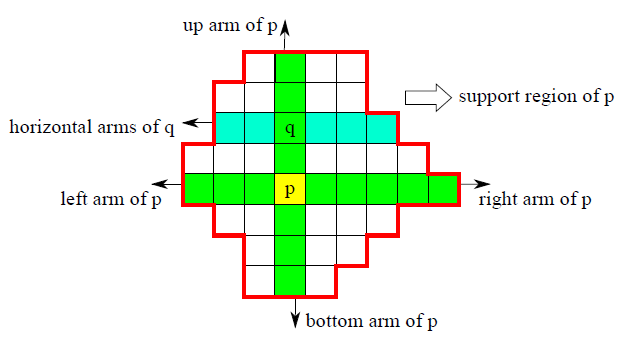
\includegraphics[scale=0.8]{Images/cost_computation.png}
	\label{cost_computation}
	\caption{ The adaptive windows only keeps pixel that have strong enough color similarities with the pixel in its center. It also has a maximum size which avoid the case of huge windows.}
\end{center}
\end{figure}

\newpage

We then define, for each pixel $p$, upward, downard, leftward and rightward borders pixel $q$ with the following algorithm. The border pixel $q$ has to be the last pixel in a given direction that is such that:
\begin{itemize}
	\item[\textbf{1. }]$D_C(q, p) < \tau_1$ and $D_C(q, q_{predecessor}) < \tau_1$
	\item[\textbf{2. }]$D_S(q, p) < L_1$
	\item[\textbf{3. }]$D_C(q, p) < \tau_2 < \tau_1$ if $L_2 <  D_S(q, p) < L_1$
\end{itemize}
where $D_C(p, q) = \max_{i \in R, G, B} |I_i(p) - I_i(q)|$ is the color distance between 2 pixels and  $D_S(p, q) = |p - q|$ is the spatial distance between 2 pixels.\\
The first condition ensures that pixels which belong to the same window have enough color similarity and that this similarity is kept from the center of the window to the edge. The second defines a limit size for the window in order to avoid too large windows that would not perform better but would cost more computation time. The last condition reduce the maximal size of the window when the region is too textured.\\
With the borders defined, the cost can be aggregated either horizontally first or vertically first. This way, two adaptive windows are defined depending on the order of aggregation. In order to get a stable cost volume, \cite{adCensus} advises us to compute the agregation 4 times, twice horizontally first and twice vertically first.\\

\begin{figure}[h]
\begin{center}	
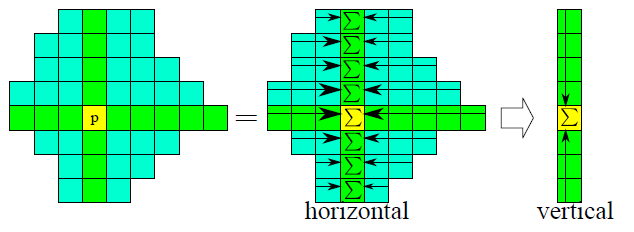
\includegraphics[scale=0.7]{Images/cost_aggregation.png}
	\label{cost_aggregation}
	\caption{ The aggregation is done one direction after the other with the corresponding border pixels.}
\end{center}
\end{figure}

\subsection{Scanline Optimization}

For better matching results, a second aggregating step is then computed. It follows the multi-direction scanline optimizer developed by \textit{Hirschmüller} in \cite{scanlineOptim}. The idea is to refine the cost along one direction by comparing the cost of the neighboring pixels and disparities.\\
Four scanline optimizations are thus processed independently, leftward, rightward, upward and downward. For a given direction $r$, the cost is updated from the first column/line to the last with the following formula:
\begin{eqnarray*}
	C_r (p, d) &=&
	 C(p, d) - \min_k C_r(p-r, k)\\
	 && + \min\left( C_r(p, d) , C_r(p-r, d+1) + P_1, C_r(p-r, d-1) + P_1, \min_k C_r(p-r, k) + P_2\right)
\end{eqnarray*}
where $p-r$ is the previous pixel along the direction $r$.\\
$P_1 < P_2$ are parameters that penalize the disparity change between neighboring pixels. They depends on $D_1 = D_C(p, p-r)$ in the left picture and $D_2 = D_C(pd, pd-r)$ in the right picture. They are symmetrically set by the formulas:
\begin{itemize}
	\item[\textbf{1. }]$P_1 = \Pi_1, \ \ P_2 = \Pi_2,$ if $D_1 < \tau_{SO}$ and $D_2 < \tau_{SO}$
	\item[\textbf{2. }]$P_1 = \frac{\Pi_1}{4}, \ \ P_2 =\frac{\Pi_2}{4},$ if $D_1 > \tau_{SO}$ and $D_2 < \tau_{SO}$
	\item[\textbf{3. }]$P_1 = \frac{\Pi_1}{4}, \ \ P_2 =\frac{\Pi_2}{4},$ if $D_1 < \tau_{SO}$ and $D_2 > \tau_{SO}$
	\item[\textbf{4. }]$P_1 = \frac{\Pi_1}{10}, \ \ P_2 =\frac{\Pi_2}{10},$ if $D_1 > \tau_{SO}$ and $D_2 > \tau_{SO}$
\end{itemize}
where $\Pi_1, \ \ \Pi_2 $ and $\tau_{SO}$ are parameters.\\
\\
Finally, the scanline optimization cost is the average of the 4 directional costs computed previously:
\[
	C(p, d) = \frac{1}{4} \sum_r C_r(p,d)
\]

\section{Disparity Refinement}

The aim of this part is to find the outliers in the disparity maps of the right and the left picture. Once they are found, their intensities are replaced by new one computed with the information found on the neighboring inliers. The original article
\cite{adCensus} proposes many methods in order to find outliers and correct their values.\\
The first one is the left-right consistency check that is commonly used for refinement. It consists of declaring outliers all the pixels whose disparity is not consistent between left and right picture:
\[
	p \text{ is declared outlier } \Leftrightarrow \text{disparity}(p) \neq \text{disparity}(p+d)
\]
However, even if \cite{adCensus} does not precise it, we consider that pixels that checks the equality above with an error of $\pm 1$ are not considered as outliers. In fact, as the disparity is an integer, many good matches would be declared as outliers.\\
The other methods of refinement presented by \cite{adCensus} did not present enough details so we use another method from \textit{REFFFFFFFFFFFFFFFF} to fill the outliers values.

\newpage

\section{Results}

\newpage

\section{Conclusion}

\newpage

\begin{thebibliography}{9}
\bibitem{middleBench}
	D. Scharstein and R. Szeliski,
	\emph{ Middlebury benchmark}.
	vision.middlebury.edu/stereo/

\bibitem{adCensus}
	X. Mei, X. Sun, M. Zhou, S. Jiao, H. Wang, and X. Zhang,
	\emph{On building an accurate stereo matching system on graphics hardware}.
	GPUCV,
	2011.

\bibitem{stereoTaxonomy}
	D. Scharstein and R. Szeliski,
   	\emph{ A taxonomy and evaluation of dense two-frame stereo correspondence algorithms}.
	International Journal of Computer Vision, 
	47(1/2/3):7-42, 
	April-June 2002.

\bibitem{costAggreg}
	K. Zhang, J. Lu, and G. Lafruit,
	\emph{ Cross-based local stereo matching using orthogonal integral images}.
	IEEE TCSVT,
	19(7):1073–1079,
	2009.
	
\bibitem{scanlineOptim}
	H. Hirschmüller,
	\emph{Stereo processing by semiglobal matching
and mutual information}.
	IEEE TPAMI,
	30(2):328–341,
	2008.

\end{thebibliography}

\end{document}
%-------------------------------------------------------------------------------
